\documentclass[border=10pt]{standalone}
\usepackage[utf8]{inputenc}

\usepackage{tikz}
\usepackage{smartdiagram}
\usetikzlibrary{positioning}
\definecolor{blue_louise}{HTML}{527AC2}
\definecolor{red_louise}{HTML}{DC2A2A}
\definecolor{green_louise}{HTML}{1BA39C}
\definecolor{purple_louise}{HTML}{2E1B36}
\definecolor{gray_louise}{HTML}{2E343B}
\tikzset
  {mybox/.style=
    {rectangle,rounded corners,drop shadow,minimum height=1cm,
     minimum width=2cm,align=center,fill=#1,draw=gray_louise,line width=1pt
    },
   myarrow/.style=
    {draw=#1,line width=3pt,-stealth,rounded corners
    },
   mylabel/.style={text=#1}
  }
\begin{document}
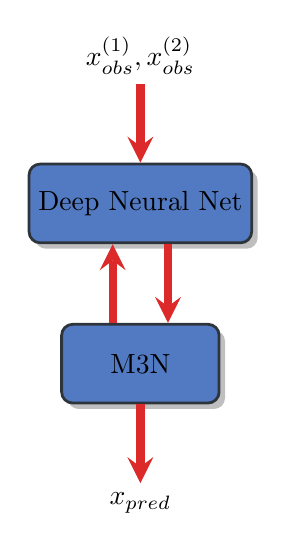
\begin{tikzpicture}
  \node (X_obs) {$x_{obs}^{(1)}, x_{obs}^{(2)}$};
  \node[mybox=blue_louise, below=of X_obs] (DNN) {Deep Neural Net};
  \node[mybox=blue_louise,below=of DNN] (M3N) {M3N};
  \node[below=of M3N] (X_pred) {$x_{pred}$};
  
  \draw[myarrow=red_louise] (X_obs)--(DNN);
  \draw[myarrow=red_louise] ([xshift=1em]DNN.south) --([xshift=1em]M3N.north);
  \draw[myarrow=red_louise] ([xshift=-1em]M3N.north) --([xshift=-1em]DNN.south);
  \draw[myarrow=red_louise] (M3N) -- (X_pred);
%  \draw[myarrow=red_louise] (CR2) -- (CR3);
%  \draw[myarrow=red_louise] (CR3) -- (PD);
%%  \draw[myarrow=gray_louise] (CR3.east) -- +(0.7,0) coordinate (VD1)
%%    -- (VD1|-CR1) coordinate (VD2) -- (CR1);
%    \draw[myarrow=gray_louise] (X_obs.east) -- +(1.7,0) coordinate (VD1)
%    -- (VD1|-PD) coordinate (VD2) -- (PD.east);
%  \draw[myarrow=red_louise] (PD) -- (X_pred);
  
%  \path (CR1) -- node[mylabel=gray_louise,left]{$6 \times M \times N$} (CR2);
%  \path (CR2) -- node[mylabel=gray_louise,left]{$6 \times M \times N$} (CR3);
%  \path (CR3) -- node[mylabel=gray_louise,left]{$2 \times M \times N$} (PD);
%  \path (VD1) -- node[mylabel=gray_louise,right]{$1 \times M \times N$} (VD2);
%  \path (VD1) -- node[mylabel=gray_louise,right]{$1 \times M \times N$} (VD2);
\end{tikzpicture}
\end{document}


\end{document}
